\documentclass[12pt]{extarticle}
\usepackage[utf8]{inputenc}
\usepackage{cite}
\usepackage{enumitem}
\usepackage{graphicx}
\usepackage{hyperref}

\title{\textbf{e-Yantra Ideas Competition 19-20}}
\author{\textbf{Project Name : }Smart Greenhouse Monitoring System}
\date{\textbf{Team Id : }1143}

\begin{document}

\maketitle
\pagenumbering{gobble}

% creating sections
\section{Introduction/Motivation : }
% Writing the paragraph
\paragraph{}
A greenhouse is a structure with walls and roof made chiefly of transparent material, such as glass, in which plants requiring regulated climatic conditions are grown[4].
\paragraph{}
Many problems are encountered during greenhouse cultivation[1]. These problems result in yield that doesn’t fulfil the international and national market standards. Thus, it results in wastage of energy and crops. 
\paragraph{}
Smart greenhouse is a concept of greenhouse that cultivates crops without human intervention. Crops in a smart greenhouse grow without adjustment of climate or any human interference by any means for a particular period. The smart greenhouse uses various microprocessors and sensors to perform functions such as controlling temperature and irrigation system. Any type of plant, fruit, and vegetables can be grown at any time of year in smart greenhouse. This system is cost effective and improves efficiency and versatility of greenhouses.
\paragraph{}
The objective is to introduce a system that effectively identifies the internal parameters of the greenhouse and monitors those parameters continuously. Also, the environmental parameters are maintained by the system according to the requirement of the plant.
\paragraph{}
Sustainable Development Goal trying to achieve :
\begin{enumerate}
    \item Industry, Innovation and Infrastructure
    \item Responsible consumption and production
\end{enumerate}


\section{Market Research/Literature Survey : }
\paragraph{}
Andrei Klubnikin[3] suggested a method in 2017 of developing a smart greenhouse monitoring using Internet of Things. Different sensors[2] are used to detect the environmental conditions and necessary actions are taken based on the data. It would help in accelerating the growth of said "ungrowable" crops[5] in controlled weather conditions.
\paragraph{}
By 2022, the global IoT greenhouse market will top $1.3 billion (up from $680 million in 2016). However, the Internet of Things applications in agriculture are not limited to connected greenhouse solutions[3]. 
\paragraph{}
Agro-based economies like India are a perfect working ground for smart agriculture and its applicability. A recent study by Statista has shown that smart agriculture is expected to take up \$26.76 billion of global market size by 2020 and Asia is expected to hold 40\% of the global market share. According to NASSCOM report, India has around 40 startups dealing in smart agriculture
\paragraph{}
Our main stakeholders are the agricultural industries and agencies and individuals that perform greenhouse cultivation.


\section{Hardware Requirements : }
% List of hardware components
% Nested list
\begin{itemize}
    \item Sensors \begin{enumerate}
        \item \textbf{Air temperature wireless sensor (indoor/outdoor):}
        
        \textbf{Sensor:} LM35 TO-92-3 Board Mount Temperature Sensor

For optimizing the aeration doors opening and closure and the fan turning on and off.
        \item \textbf{Air humidity wireless sensor (indoor/outdoor):}
        
        \textbf{Sensor:} DHT22/AM2302 Digital Temperature and Humidity Sensor

For optimizing the aeration doors opening and closure and the fan turning on and off.
        
        \item \textbf{Air Quality detector(indoor):}
        
        \textbf{Sensor:} MQ135 Air Quality Gas Sensor Module

For detecting the presence of harmful gases

        \item \textbf{Soil moisture wireless sensor:}
        
        \textbf{Sensor:} Three-Way Soil Meter For Moisture,Light Intensity and pH Testing Meter

For optimizing the irrigation.

        \item \textbf{Brightness wireless sensor:}
        
        \textbf{Sensor:} CJMCU-TEMT6000

For optimizing the use of shading net.

        \item \textbf{EC electrical conductivity:}
        
        \textbf{Sensor:} Conductivity/TDS /Salinity Cell

For measuring the soil conductivity which is useful for optimizing the fertigation.

        \item \textbf{pH sensor:}
        
        \textbf{Sensor:} Three-Way Soil Meter For Moisture,Light Intensity and pH Testing Meter

For optimizing the fertigation.

        \item \textbf{Anemometer:}
        
        \textbf{Sensor:} Wind Speed meter

To control the wind speed during the aeration doors opening.

        \item \textbf{Camera Module:}
        
        \textbf{Sensor:} Raspberry Pi Camera

For remote surveillance

        \item \textbf{Grove Soil Moisture:}
        
        \textbf{Sensor:} R6010 Pinless Moisture Meter

Utilized to recognize the dampness of soil or judge if there is water around the sensor, let the plants inside greenhouse connect for human help.

    \end{enumerate} 
    
    \item Actuators \begin{enumerate}
        \item \textbf{Wireless relays module:}
        
For on/off lighting, irrigation pumps.

        \item \textbf{Mosfet/PWM module:}
        
For varying intensity,heating,heat and light

    \end{enumerate}

    \item Raspberry Pi

    \item Arduino Uno
\end{itemize}

\section{Software Requirements : }
% List of softwares required
\begin{enumerate}
    \item Python 3.7.x
    \item Arduino IDE
    \item APIs
    \item Mobile App / Web
    \item Server / Cloud
\end{enumerate}

\section{Implementation : }
\subsection{Setting Up of the System :}
%Vignesh Code Starts
    \begin{enumerate}[label=\alph*]
        \item 
        The crop requires different conditions at different times of the day and in different months. A dataset of all the ranges of different parameters is developed. This dataset is then loaded onto the system.\\\\
        Different parameters that are monitored are :
            \begin{enumerate}
                \item Air temperature, Humidity, Quality
                \item Soil Humidity, pH
                \item Light Intensity
            \end{enumerate}
        \item
        Sensors for measuring air humidity, temperature, quality and light intensity are placed at a vertical height. The actuators for the same are also placed along the vertical height of the greenhouse. The soil sensors are placed within the soil.\\
        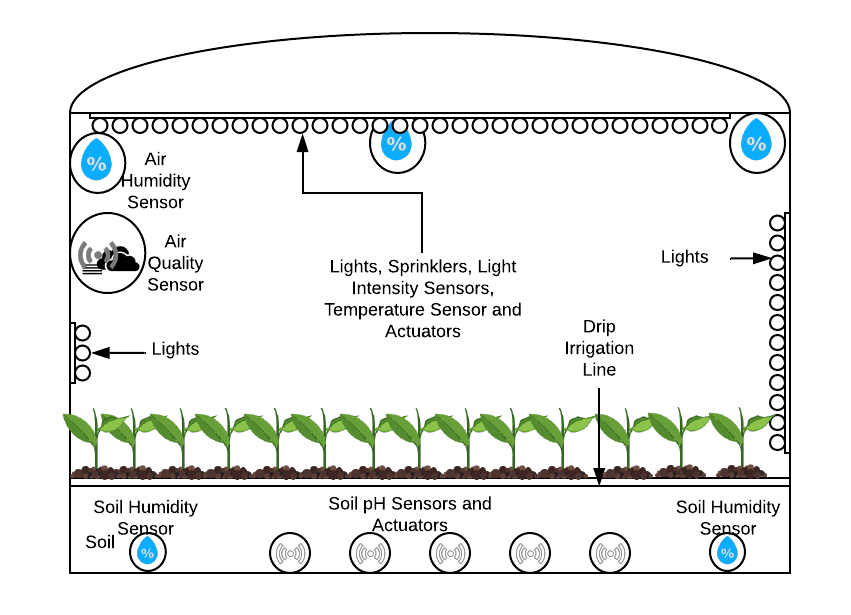
\includegraphics[width=13cm]{sensors.png}
    \end{enumerate}
%Vignesh Code ends
\subsection{Greenhouse Monitoring and Maintenance :}
%Vignesh Code Starts
    \begin{enumerate}[label=\alph*]
        \item
            \textbf{Collecting Data}\\
            The different sensors continuously sense the environment and this data is sent to RaspberryPi in the form of electrical signals.
        \item
            \textbf{Analysis}\\
            The data received from various sensors is then analysed to take further action. Different parameters are analysed differently.\\\\
            \textbf{Air and Soil Humidity}\\
            Different values of humidity for every hour of the day is recorded. The air and soil humidity together decide how much irrigation is required for the plant.\\\\
            Moisture is majorly affected by the temperature and transpiration rate of the plant.\\
            The transpiration rate of the plant varies in different seasons.
            \begin{enumerate}[label=\arabic*]
                \item
                On  a normal day, the transpiration rate is normal and humidity never crosses the threshold.
                \item
                On rainy days or in the winter or on cloudy days, the plant doesn’t transpire a lot. Thus, the transpiration rate is low. But during these seasons, the air moisture is high. Hence, the plant has sufficient water and frequent irrigations are to be avoided.
                \item
                In the summer season, the transpiration rate is high and the overall moisture is less. Thus, the air moisture is low as well as the soil moisture. So, more frequent irrigation is required.
                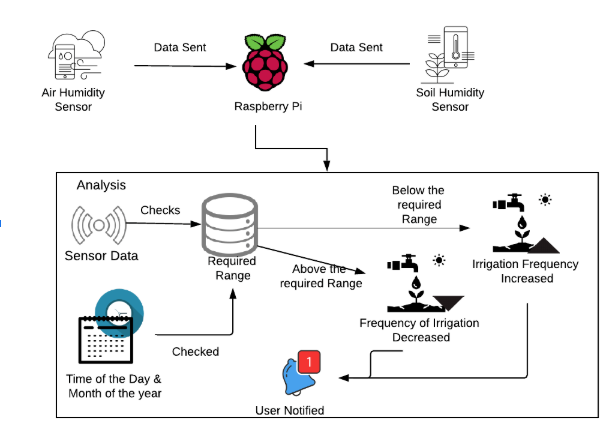
\includegraphics[width=12cm]{Maintenance.png}
                \begin{center}
                    Analysis of Soil and Air Humidity\\
                \end{center}
            \end{enumerate}
            \textbf{Air Temperature:}\\
            The sensor data for air temperature is analysed as follows :-
            \begin{enumerate}[label=\arabic*]
                \item
                The time of the day and the month of the year is checked. Depending on this value, the ideal range temperature is fetched/calculated by the system.
                \item
                The received data is checked with this range. If it falls within the range, then no action is required.
                \item
                If the air temperature is high, then the sprinklers(that hang from the roof of the greenhouse) are started. While these sprinklers are working, the humidity within the greenhouse is also maintained.
                \item
                If the air temperature is low, then the heaters are switched on. While the heaters are working, the temperature and moisture within the greenhouse are monitored and it is checked that none of the parameters go disarray.
            \end{enumerate}
            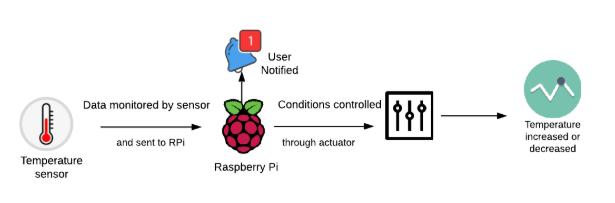
\includegraphics[width=12cm]{AirTemp.png}
            \begin{center}
                Analysis and Maintenance of Air Temperature\\
            \end{center}
            \textbf{Light Intensity:}
            \\Light Intensity depends on time of the day and the month / season. The received data is checked to be within a required range. This range is decided according to the time of the day and the season.
                \begin{enumerate}[label=\arabic*]
                    \item
                    During a sunny day, the intensity will never fall below the required range. It will only be above a certain limit. In case of high light intensity, the artificial lights are switched off and if required the shades are pulled close.
                    \item
                    During monsoon and winter, the intensity may fall below the required range. In case of low intensity, lights are within the greenhouse are switched on if it is night or if it is a cloudy day. On a sunny day the shades are opened and the sunlight is used for increasing the intensity.
                    \begin{center}                        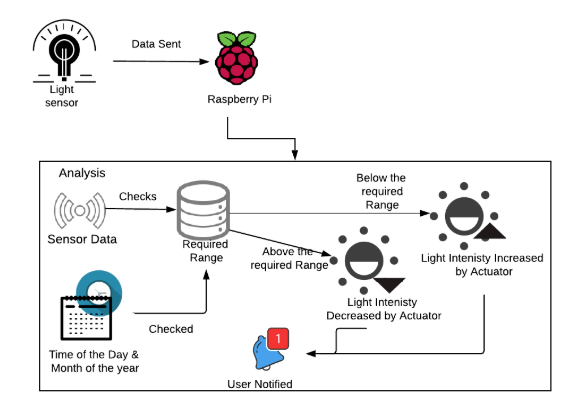
\includegraphics[width=12cm]{LightIntensity.png}
                        Analysis and Maintenance of Light Intensity\\
                    \end{center}
                \end{enumerate}
            \textbf{Other Parameters:}\\
            Air quality and soil ph is analysed based on various parameters and the user is accordingly notified about the alarming levels of each parameter.
            \begin{center}
                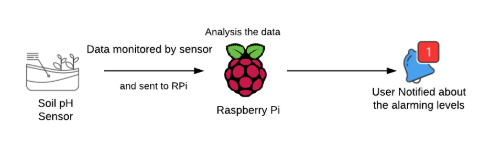
\includegraphics[width=12cm]{SoilpH.png}
                Soil pH Monitoring
                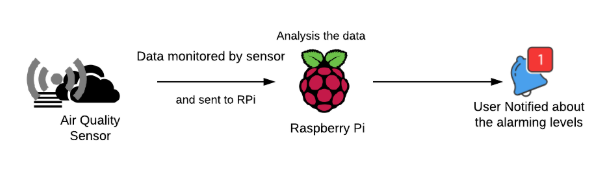
\includegraphics[width=12cm]{AirQuality.png}
                Air Quality Monitoring
            \end{center}
    \end{enumerate}
    \begin{center}
        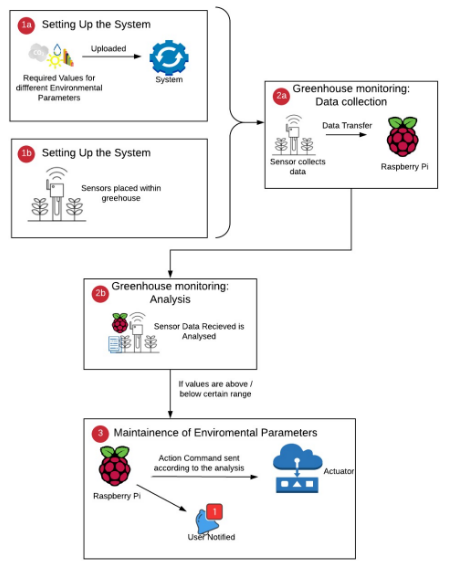
\includegraphics[width=12cm,height=14cm]{FlowDiagram.png}
    \end{center}
    \begin{center}
        Flow Diagram
    \end{center}
%Vignesh Code Ends
\section{Feasibility : }
\paragraph{}
Present systems require manual monitoring of the greenhouse parameters. This causes a lot of problems and even increases the workload. To overcome the problems encountered during manual monitoring, we propose an automated monitoring system. In this, all the environmental parameters are monitored and maintained well. The crop yield is according to the international market standards. Thus, this solution is feasible.
\paragraph{}
While constructing a greenhouse, sensors for temperature and air quality are put up. Only a few extra sensors will have to wired along with actuators. The user will use app. Thus, this solution is also cost-effective. It is cost effective as the total estimated cost and the turnover expected after the introduction of a smart warehouse is much more than what traditional farming could provide, thus increasing profit for the farmer on his investment.
\begin{thebibliography}{9}
    \bibitem{1}
    Greenhouse Cultivation: Problems and Solutions [Online]\\
    Link:\href{https://www.auroras.eu/greenhouse-cultivation-problems-and-solutions/}{https://www.auroras.eu/greenhouse-cultivation-problems-and-solutions/} [20th Oct 2019]
    \bibitem{2}
    Greenhouse: the integrated solution for greenhouses\\
    Link:\href{https://www.auroras.eu/green-house-the-integrated-solution-for-greenhouses/}{https://www.auroras.eu/green-house-the-integrated-solution-for-greenhouses/} [21st Oct 2019]
    \bibitem{3}
    Andrei Kulbnikin on Iot Agriculture : How to Build a greenhouse?(2017)\\
    Link:\href{https://r-stylelab.com/company/blog/iot/iot-agriculture-how-to-build-smart-greenhouse}{https://r-stylelab.com/company/blog/iot/iot-agriculture-how-to-build-smart-greenhouse} [22nd Oct 2019]
    \bibitem{4}
    Greenhouse\\
    Link:\href{https://en.wikipedia.org/wiki/Greenhouse}{https://en.wikipedia.org/wiki/Greenhouse} [12th Sept 2019]
    \bibitem{5}
    GreenHouse helping Farmers to grow Crops\\
    Link:\href{https://www.fastcompany.com/40405369/this-low-cost-greenhouse-is-designed-to-help-the-poorest-farmers}{https://www.fastcompany.com/40405369/this-low-cost-greenhouse-is-designed-to-help-the-poorest-farmers} [20th Sept 2019]
    \bibitem{6}
    GreenHouse Farming Worldwide Market\\
    Link:\href{http://www.sourcetrace.com/productivity-control-greenhouse-farming/}{http://www.sourcetrace.com/productivity-control-greenhouse-farming/} [20th Sept 2019]
\end{thebibliography}
% \bibliography{References}
    % \begin{enumerate}[label=\arabic*]
    %     \item
    %     Greenhouse Cultivation: Problems and Solutions [Online]\\ Link : \href{https://www.auroras.eu/greenhouse-cultivation-problems-and-solutions/}{https://www.auroras.eu/greenhouse-cultivation-problems-and-solutions/} [20th Oct 2019]
    %     \item
    %     Greenhouse: the integrated solution for greenhouses\\
    %     Link : \href{https://www.auroras.eu/green-house-the-integrated-solution-for-greenhouses/}{https://www.auroras.eu/green-house-the-integrated-solution-for-greenhouses/} [21st Oct 2019]
    %     \item
    %     Andrei Kulbnikin on Iot Agriculture : How to Build a greenhouse ? (2017)\\
    %     Link : \href{https://r-stylelab.com/company/blog/iot/iot-agriculture-how-to-build-smart-greenhouse}{https://r-stylelab.com/company/blog/iot/iot-agriculture-how-to-build-smart-greenhouse} [22nd Oct 2019]
    %     \item
    %     Greenhouse\\
    %     Link : \href{https://en.wikipedia.org/wiki/Greenhouse}{https://en.wikipedia.org/wiki/Greenhouse} [12th Sept 2019]
    %     \item
    %     GreenHouse helping Farmers to grow Crops\\
    %     Link: \href{https://www.fastcompany.com/40405369/this-low-cost-greenhouse-is-designed-to-help-the-poorest-farmers}{https://www.fastcompany.com/40405369/this-low-cost-greenhouse-is-designed-to-help-the-poorest-farmers} [20th Sept 2019]
    %     \item
    %     GreenHouse Farming Worldwide Market\\
    %     Link : \href{http://www.sourcetrace.com/productivity-control-greenhouse-farming/}{http://www.sourcetrace.com/productivity-control-greenhouse-farming/} [20th Sept 2019]
    % \end{enumerate}
\end{document}
